\documentclass[12pt,a4paper,titlepage]{article}

\usepackage{xcolor}
\usepackage{minted}
\usepackage{titlesec}
\usepackage{graphicx}
\usepackage[portuguese]{babel}
\usepackage[colorlinks=true,allcolors=black]{hyperref}

\graphicspath{ {./img/}{./../der/}{./../relacional} }

\newcommand{\sql}{./../sql/}
\newcommand{\sectionbreak}{\clearpage}
\setminted{
    linenos=true,
    style=default,
    frame=single,
    framesep=3mm,
    breaklines=true,
    fontsize=\small,
    tabsize=4,
    numbersep=5pt,
    autogobble=true
}

\title{Trabalho Prático - Banco de Dados}
\author{
    
\includegraphics[scale=0.28]{./../../../../puc.png}
    \\[1.5em]
    \\Fernando de Lima Gonçalves
    \\Igor Luiz Santos de Lima
    \\Laura Martins de Souza
    \\Matheus de Oliveira Chaves Teixeira
}
\date{Belo Horizonte\\2026}

\begin{document}
\maketitle
\tableofcontents

\section{Modelos e Diagramas}
\subsection{Entidade-Relacionamento}
\begin{figure}[h]
    \center
    \caption{DER Trabalho Prático}
    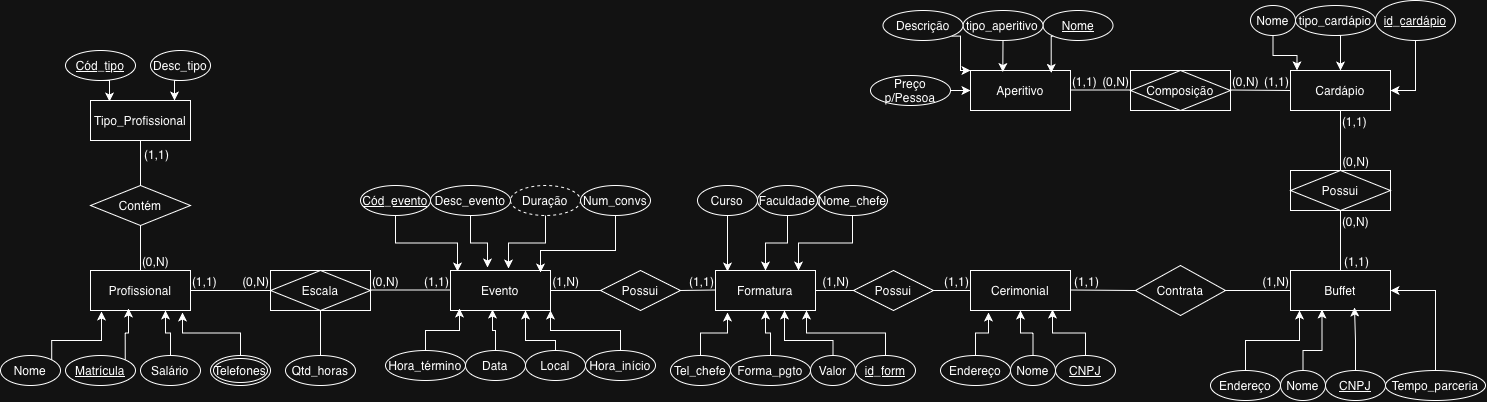
\includegraphics[width=\textwidth]{der}
    \\\small{Elaborado pelos integrantes do grupo}
    \label{fig:der}
\end{figure}

\clearpage\subsection{Relacional}
\begin{figure}[h]
    \center
    \caption{DR Trabalho Prático}
    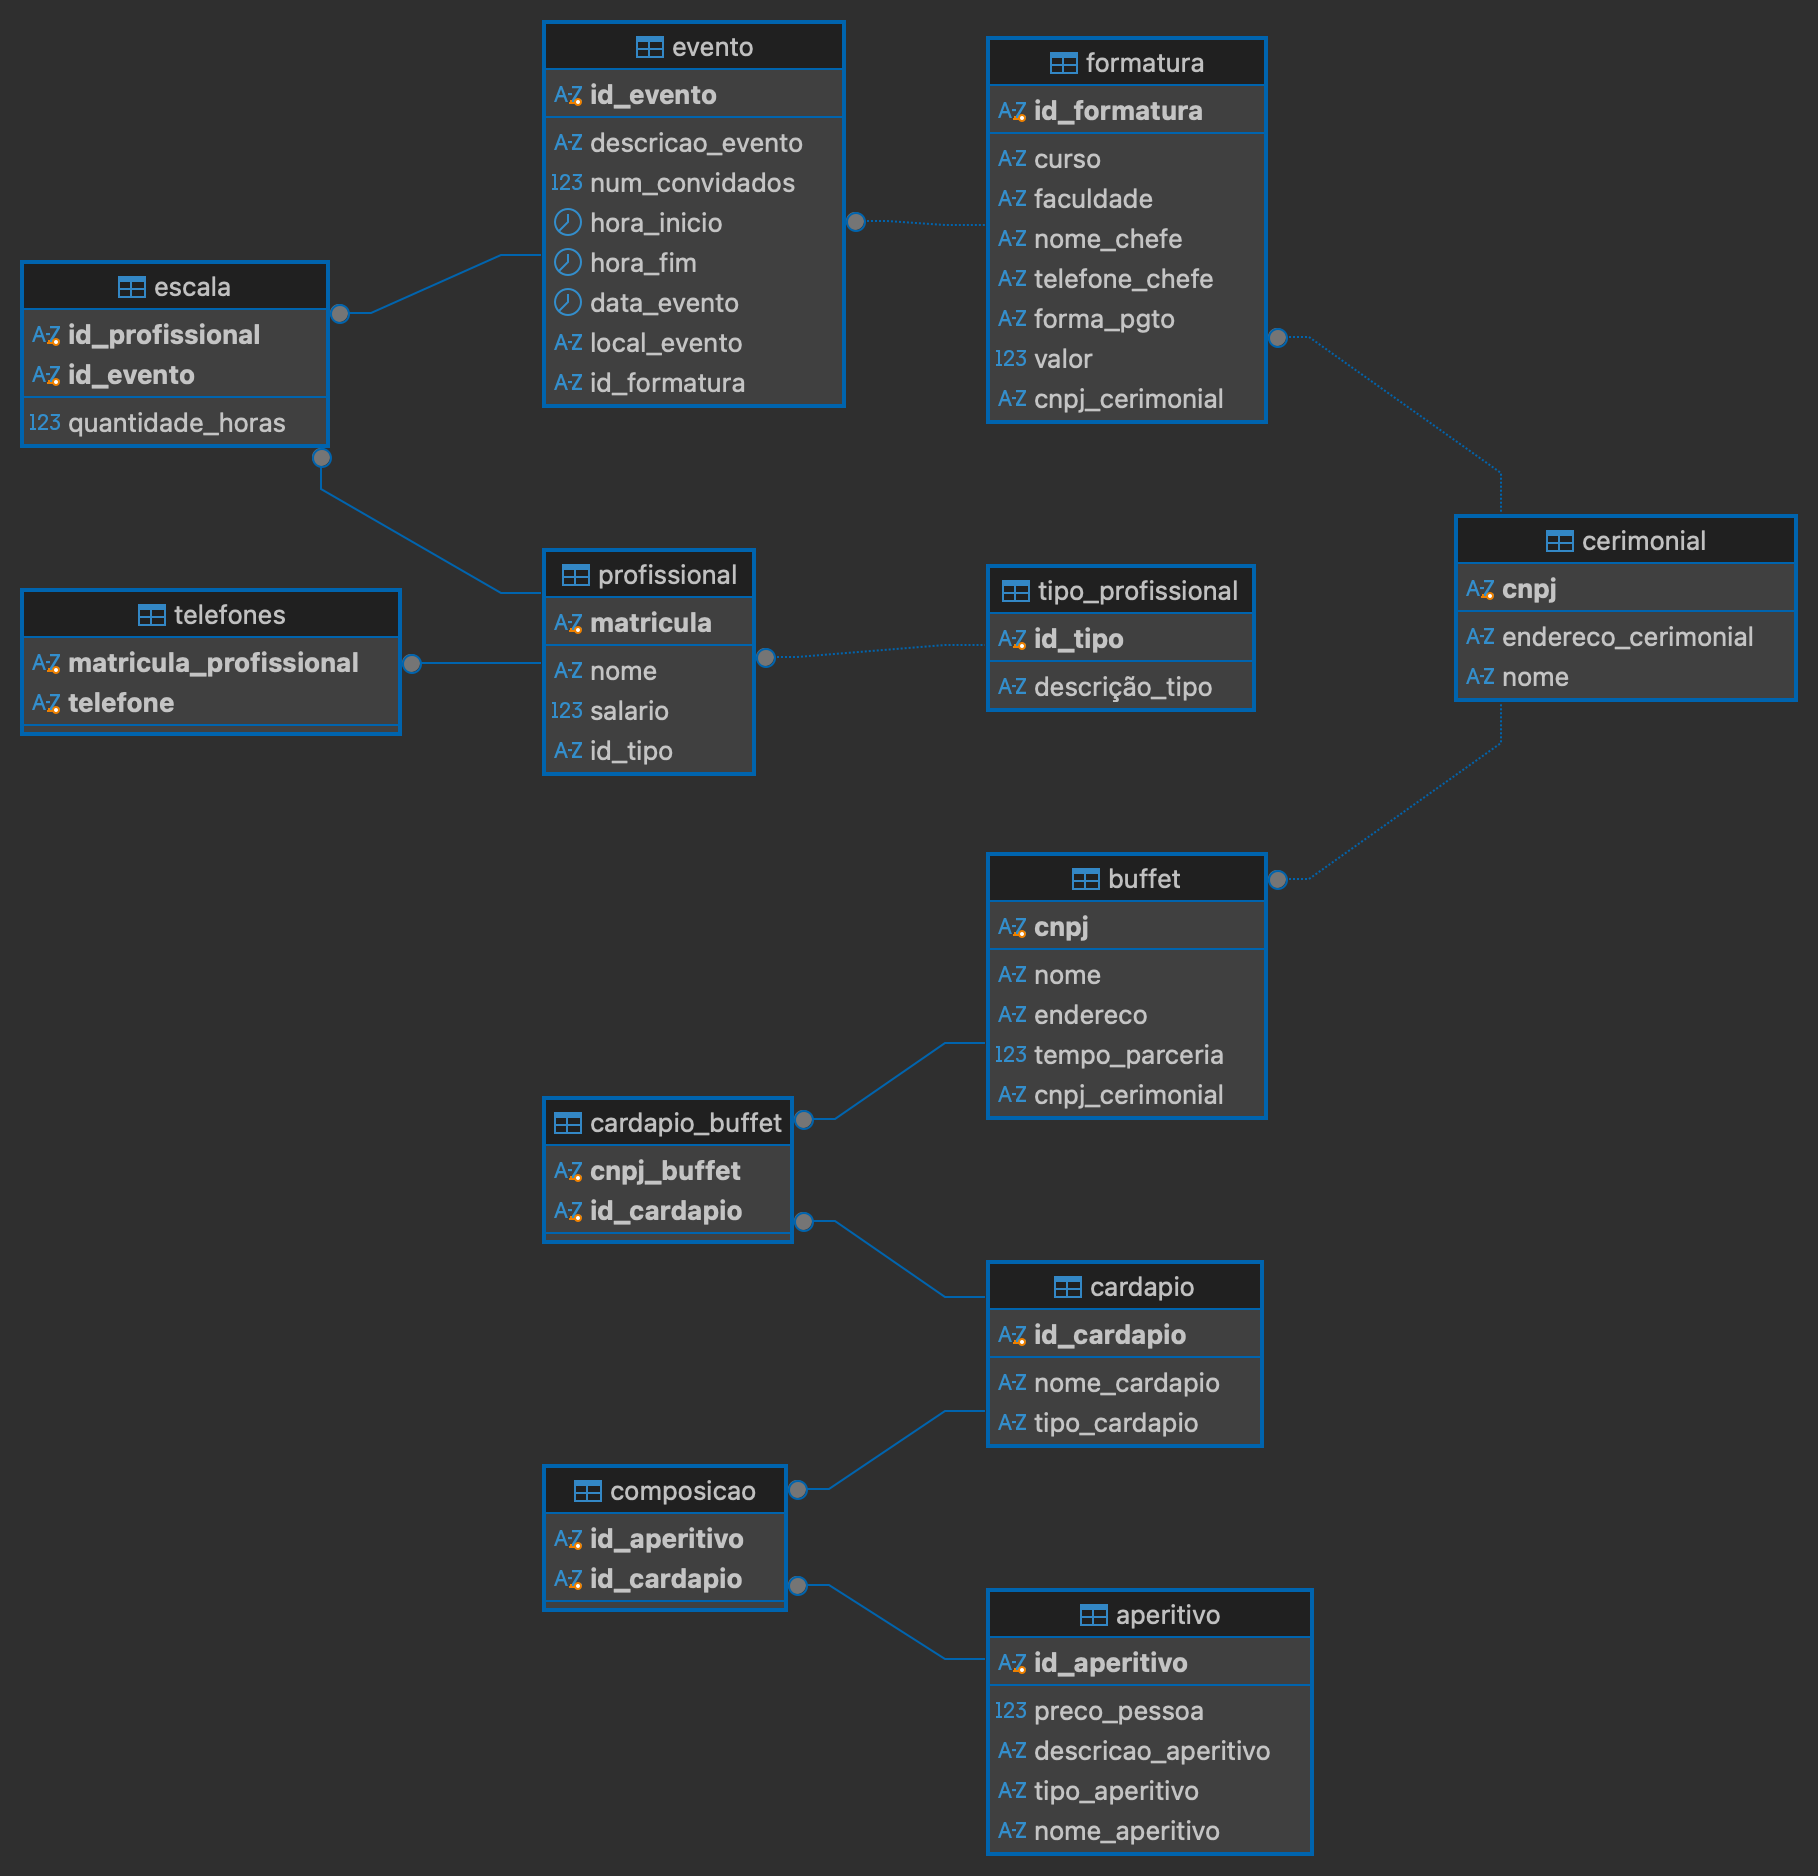
\includegraphics[width=\textwidth]{relacional}
    \\\small{Elaborado pelos integrantes do grupo}
    \label{fig:dr}
\end{figure}

\section{Scripts SQL}
\subsection{Banco de Dados}
\inputminted{sql}{\sql ini.sql}

\clearpage\subsection{Povoamento}
\inputminted{sql}{\sql povoar_4_cerimoniais.sql}

\end{document}
